\documentclass[aspectratio=169,11pt]{beamer}

% TEMA Y COLORES
\usetheme{Madrid}
\usecolortheme{whale}

\definecolor{primaryblue}{RGB}{0,102,153}
\definecolor{accentgreen}{RGB}{0,128,0}
\definecolor{accentorange}{RGB}{204,102,0}
\definecolor{darkgray}{RGB}{64,64,64}

\setbeamercolor{palette primary}{bg=primaryblue,fg=white}
\setbeamercolor{palette secondary}{bg=primaryblue!80,fg=white}
\setbeamercolor{palette tertiary}{bg=primaryblue!60,fg=white}
\setbeamercolor{structure}{fg=primaryblue}
\setbeamercolor{block title}{bg=primaryblue,fg=white}
\setbeamercolor{block body}{bg=primaryblue!10}
\setbeamercolor{block title example}{bg=accentgreen,fg=white}
\setbeamercolor{block body example}{bg=accentgreen!10}
\setbeamercolor{block title alerted}{bg=accentorange,fg=white}
\setbeamercolor{block body alerted}{bg=accentorange!10}

% PAQUETES
\usepackage[utf8]{inputenc}
\usepackage[T1]{fontenc}
\usepackage{amsmath,amssymb}
\usepackage{booktabs}
\usepackage{tikz}
\usepackage{pgfplots}
\usepackage{listings}
\usepackage{multicol}

\pgfplotsset{compat=1.17}
\lstset{literate={ñ}{{\~n}}1 {á}{{\'a}}1 {é}{{\'e}}1 {í}{{\'i}}1 {ó}{{\'o}}1 {ú}{{\'u}}1}

% CÓDIGO PYTHON
\lstdefinestyle{pythonstyle}{
    language=Python,
    basicstyle=\ttfamily\footnotesize,
    keywordstyle=\color{blue}\bfseries,
    stringstyle=\color{red},
    commentstyle=\color{accentgreen}\itshape,
    frame=single,
    breaklines=true,
    showstringspaces=false,
    backgroundcolor=\color{gray!10}
}

% NAVEGACIÓN Y PIE DE PÁGINA
\setbeamertemplate{navigation symbols}{}
\setbeamertemplate{footline}{
    \leavevmode%
    \hbox{%
        \begin{beamercolorbox}[wd=.333333\paperwidth,ht=2.25ex,dp=1ex,center]{author in head/foot}%
            \usebeamerfont{author in head/foot}Matemáticas Financieras
        \end{beamercolorbox}%
        \begin{beamercolorbox}[wd=.333333\paperwidth,ht=2.25ex,dp=1ex,center]{title in head/foot}%
            \usebeamerfont{title in head/foot}Sesión 7
        \end{beamercolorbox}%
        \begin{beamercolorbox}[wd=.333333\paperwidth,ht=2.25ex,dp=1ex,right]{date in head/foot}%
            \usebeamerfont{date in head/foot}\insertframenumber{} / \inserttotalframenumber\hspace*{2ex}
        \end{beamercolorbox}}%
    \vskip0pt%
}

\title[Sesión 7]{Amortización de Préstamos}
\subtitle{Sistemas de pago de deuda}
\author{Matemáticas Financieras}
\institute{Valor del Dinero en el Tiempo}
\date{Semana 4 | Clase 1 | Duración: 1h 50min}

\begin{document}

% ===========================================
% SECCIÓN 1: PORTADA Y CONTENIDO
% ===========================================

\begin{frame}
    \titlepage
\end{frame}

\begin{frame}{Contenido de la Sesión}
    \tableofcontents
\end{frame}

% ===========================================
% SECCIÓN 2: INTRODUCCIÓN
% ===========================================
\section{Introducción}

\begin{frame}{Conexión con las Sesiones Anteriores}
    \begin{block}{Sesiones 5 y 6: Anualidades}
        Aprendimos que un préstamo con cuota fija es una \textbf{anualidad ordinaria}:
        \[
        PV = PMT \cdot \frac{1-(1+r)^{-n}}{r}
        \]
        Y calculamos el pago mensual.
    \end{block}

    \pause
    \vspace{0.3cm}

    \begin{alertblock}{Pero surgen preguntas...}
        \begin{itemize}
            \item ¿Qué parte del pago es interés y qué parte es capital?
            \item ¿Cuánto debo después de 12 pagos?
            \item ¿Existen otras formas de estructurar un préstamo?
        \end{itemize}
    \end{alertblock}
\end{frame}

\begin{frame}{Objetivos de Aprendizaje}
    Al finalizar esta sesión, serás capaz de:
    \begin{enumerate}
        \item Construir tablas de amortización completas
        \item Calcular el saldo insoluto en cualquier momento
        \item Separar cada pago en componente de interés y capital
        \item Comparar los tres sistemas de amortización principales
        \item Analizar el impacto de pagos anticipados
        \item Usar la HP 17bII+ para cálculos de amortización
    \end{enumerate}
\end{frame}

\begin{frame}{¿Qué es la Amortización?}
    \begin{block}{Definición}
        \textbf{Amortización} es el proceso de pagar una deuda mediante pagos periódicos que incluyen:
        \begin{itemize}
            \item \textbf{Interés:} Costo del dinero prestado
            \item \textbf{Amortización del capital:} Reducción del saldo adeudado
        \end{itemize}
    \end{block}

    \pause
    \vspace{0.3cm}

    \textbf{Ecuación fundamental:}
    \[
    \boxed{\text{Pago} = \text{Interés} + \text{Amortización del Capital}}
    \]

    \pause
    \vspace{0.3cm}

    \begin{exampleblock}{Nota importante}
        El interés siempre se calcula sobre el \textbf{saldo insoluto} (lo que aún se debe), no sobre el monto original.
    \end{exampleblock}
\end{frame}

% ===========================================
% SECCIÓN 3: SISTEMA FRANCÉS
% ===========================================
\section{Sistema Francés (Cuota Fija)}

\begin{frame}{Sistema Francés: Características}
    \begin{block}{Definición}
        En el \textbf{sistema francés}, el pago total es \textbf{constante} en cada período. Es el sistema más común en préstamos hipotecarios y de consumo.
    \end{block}

    \pause
    \vspace{0.3cm}

    \textbf{Características:}
    \begin{itemize}
        \item Cuota fija: $PMT = PV \cdot \frac{r}{1-(1+r)^{-n}}$
        \item Al inicio: más interés, menos capital
        \item Al final: menos interés, más capital
        \item El saldo decrece de forma exponencial
    \end{itemize}

    \pause
    \vspace{0.3cm}

    \begin{alertblock}{Ventaja práctica}
        Facilita la planificación financiera porque el pago es predecible.
    \end{alertblock}
\end{frame}

\begin{frame}{Sistema Francés: Cálculos Período a Período}
    Para el período $t$:

    \pause
    \vspace{0.3cm}

    \textbf{Interés del período:}
    \[
    I_t = \text{Saldo}_{t-1} \times r
    \]

    \pause
    \textbf{Amortización del capital:}
    \[
    A_t = PMT - I_t
    \]

    \pause
    \textbf{Nuevo saldo:}
    \[
    \text{Saldo}_t = \text{Saldo}_{t-1} - A_t
    \]

    \pause
    \vspace{0.3cm}

    \begin{exampleblock}{Observación}
        Como el saldo disminuye, $I_t$ disminuye y $A_t$ aumenta con el tiempo (pero su suma $PMT$ es constante).
    \end{exampleblock}
\end{frame}

\begin{frame}{Ejemplo: Tabla de Amortización Francesa}
    \textbf{Préstamo:} \$100,000 | \textbf{Tasa:} 10\% anual | \textbf{Plazo:} 5 años

    \pause
    \vspace{0.2cm}

    \textbf{Cuota anual:} $PMT = 100,000 \times \frac{0.10}{1-(1.10)^{-5}} = \$26,379.75$

    \pause
    \vspace{0.3cm}

    \begin{center}
    \scriptsize
    \begin{tabular}{@{}cccccc@{}}
        \toprule
        Año & Saldo Inicial & Pago & Interés & Capital & Saldo Final \\
        \midrule
        1 & \$100,000.00 & \$26,379.75 & \$10,000.00 & \$16,379.75 & \$83,620.25 \\
        2 & \$83,620.25 & \$26,379.75 & \$8,362.02 & \$18,017.72 & \$65,602.53 \\
        3 & \$65,602.53 & \$26,379.75 & \$6,560.25 & \$19,819.50 & \$45,783.03 \\
        4 & \$45,783.03 & \$26,379.75 & \$4,578.30 & \$21,801.45 & \$23,981.59 \\
        5 & \$23,981.59 & \$26,379.75 & \$2,398.16 & \$23,981.59 & \$0.00 \\
        \midrule
        & \textbf{Total} & \$131,898.73 & \$31,898.73 & \$100,000.00 & \\
        \bottomrule
    \end{tabular}
    \end{center}
\end{frame}

\begin{frame}{Saldo Insoluto: Fórmula Directa}
    No necesitamos calcular período por período. Hay una fórmula directa:

    \pause
    \vspace{0.3cm}

    \begin{block}{Saldo Insoluto después de $k$ pagos}
        \[
        \boxed{\text{Saldo}_k = PV \cdot \frac{(1+r)^n - (1+r)^k}{(1+r)^n - 1}}
        \]

        O equivalentemente:
        \[
        \text{Saldo}_k = PMT \cdot \frac{1 - (1+r)^{-(n-k)}}{r}
        \]
    \end{block}

    \pause
    \vspace{0.3cm}

    \begin{exampleblock}{Interpretación de la segunda fórmula}
        El saldo es el VP de los pagos \textbf{restantes} ($n-k$ pagos).
    \end{exampleblock}
\end{frame}

\begin{frame}{Ejemplo: Saldo Insoluto}
    \begin{block}{Problema}
        Préstamo de \$200,000 a 10 años, 8\% anual, pagos anuales. ¿Cuál es el saldo después del pago 6?
    \end{block}

    \pause
    \vspace{0.3cm}

    \textbf{Cuota anual:}
    \begin{align*}
        PMT = 200,000 \times \frac{0.08}{1-(1.08)^{-10}} = \$29,805.86
    \end{align*}

    \pause
    \textbf{Saldo después del pago 6 (quedan 4 pagos):}
    \begin{align*}
        \text{Saldo}_6 &= PMT \times \frac{1-(1.08)^{-4}}{0.08} \\
        &= 29,805.86 \times 3.3121 = \$98,745.84
    \end{align*}
\end{frame}

% ===========================================
% SECCIÓN 4: SISTEMA ALEMÁN
% ===========================================
\section{Sistema Alemán (Amortización Constante)}

\begin{frame}{Sistema Alemán: Características}
    \begin{block}{Definición}
        En el \textbf{sistema alemán}, la amortización del capital es \textbf{constante} en cada período. El pago total disminuye con el tiempo.
    \end{block}

    \pause
    \vspace{0.3cm}

    \textbf{Características:}
    \begin{itemize}
        \item Amortización constante: $A = \frac{PV}{n}$
        \item Cuota decreciente: $\text{Pago}_t = A + I_t$
        \item Más interés total que sistema francés (pero menos al inicio)
        \item Pagos más altos al principio
    \end{itemize}

    \pause
    \vspace{0.3cm}

    \begin{alertblock}{Uso común}
        Préstamos corporativos y algunos créditos hipotecarios en Europa.
    \end{alertblock}
\end{frame}

\begin{frame}{Sistema Alemán: Cálculos}
    \textbf{Amortización por período (constante):}
    \[
    A = \frac{PV}{n}
    \]

    \pause
    \textbf{Saldo después del pago $t$:}
    \[
    \text{Saldo}_t = PV - t \cdot A = PV \left(1 - \frac{t}{n}\right)
    \]

    \pause
    \textbf{Interés en el período $t$:}
    \[
    I_t = \text{Saldo}_{t-1} \times r = PV \left(1 - \frac{t-1}{n}\right) \times r
    \]

    \pause
    \textbf{Pago en el período $t$:}
    \[
    \text{Pago}_t = A + I_t
    \]
\end{frame}

\begin{frame}{Ejemplo: Tabla de Amortización Alemana}
    \textbf{Préstamo:} \$100,000 | \textbf{Tasa:} 10\% anual | \textbf{Plazo:} 5 años

    \pause
    \vspace{0.2cm}

    \textbf{Amortización anual:} $A = 100,000 / 5 = \$20,000$

    \pause
    \vspace{0.3cm}

    \begin{center}
    \scriptsize
    \begin{tabular}{@{}cccccc@{}}
        \toprule
        Año & Saldo Inicial & Pago & Interés & Capital & Saldo Final \\
        \midrule
        1 & \$100,000 & \$30,000 & \$10,000 & \$20,000 & \$80,000 \\
        2 & \$80,000 & \$28,000 & \$8,000 & \$20,000 & \$60,000 \\
        3 & \$60,000 & \$26,000 & \$6,000 & \$20,000 & \$40,000 \\
        4 & \$40,000 & \$24,000 & \$4,000 & \$20,000 & \$20,000 \\
        5 & \$20,000 & \$22,000 & \$2,000 & \$20,000 & \$0 \\
        \midrule
        & \textbf{Total} & \$130,000 & \$30,000 & \$100,000 & \\
        \bottomrule
    \end{tabular}
    \end{center}

    \pause
    \textbf{Comparación:} Sistema francés pagó \$31,899 de interés vs. \$30,000 del alemán.
\end{frame}

% ===========================================
% SECCIÓN 5: SISTEMA AMERICANO
% ===========================================
\section{Sistema Americano (Bullet)}

\begin{frame}{Sistema Americano: Características}
    \begin{block}{Definición}
        En el \textbf{sistema americano} (o ``bullet''), solo se pagan \textbf{intereses} durante la vida del préstamo. El \textbf{principal completo} se paga al vencimiento.
    \end{block}

    \pause
    \vspace{0.3cm}

    \textbf{Características:}
    \begin{itemize}
        \item Pagos periódicos: solo interés $= PV \times r$
        \item Pago final: Principal completo $PV$
        \item Mayor pago total de intereses
        \item Saldo insoluto constante hasta el final
    \end{itemize}

    \pause
    \vspace{0.3cm}

    \begin{alertblock}{Uso común}
        Bonos corporativos, algunos préstamos puente, créditos para desarrollo inmobiliario.
    \end{alertblock}
\end{frame}

\begin{frame}{Ejemplo: Sistema Americano}
    \textbf{Préstamo:} \$100,000 | \textbf{Tasa:} 10\% anual | \textbf{Plazo:} 5 años

    \pause
    \vspace{0.3cm}

    \begin{center}
    \scriptsize
    \begin{tabular}{@{}cccccc@{}}
        \toprule
        Año & Saldo Inicial & Pago & Interés & Capital & Saldo Final \\
        \midrule
        1 & \$100,000 & \$10,000 & \$10,000 & \$0 & \$100,000 \\
        2 & \$100,000 & \$10,000 & \$10,000 & \$0 & \$100,000 \\
        3 & \$100,000 & \$10,000 & \$10,000 & \$0 & \$100,000 \\
        4 & \$100,000 & \$10,000 & \$10,000 & \$0 & \$100,000 \\
        5 & \$100,000 & \$110,000 & \$10,000 & \$100,000 & \$0 \\
        \midrule
        & \textbf{Total} & \$150,000 & \$50,000 & \$100,000 & \\
        \bottomrule
    \end{tabular}
    \end{center}

    \pause
    \vspace{0.3cm}

    \textbf{Comparación de intereses totales:}
    \begin{itemize}
        \item Francés: \$31,899
        \item Alemán: \$30,000
        \item Americano: \$50,000
    \end{itemize}
\end{frame}

% ===========================================
% SECCIÓN 6: COMPARACIÓN DE SISTEMAS
% ===========================================
\section{Comparación de Sistemas}

\begin{frame}{Comparación Visual: Pagos}
    \begin{center}
        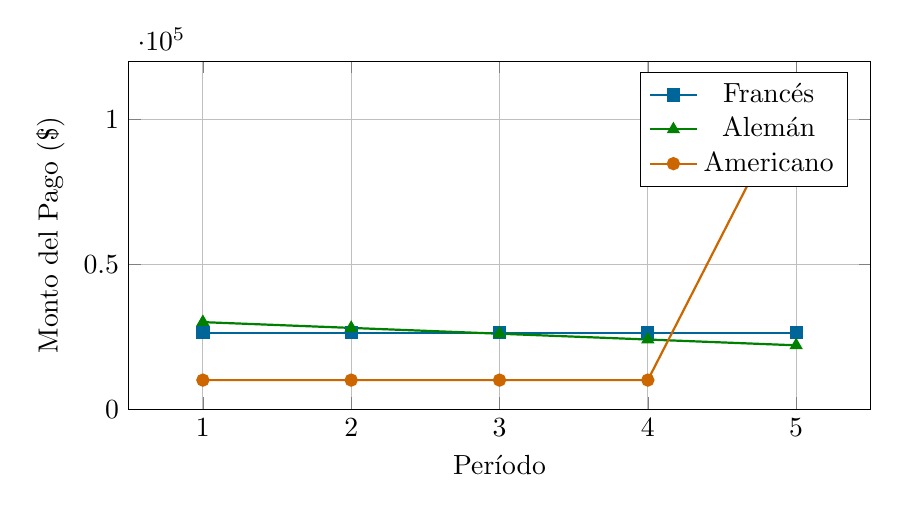
\begin{tikzpicture}
            \begin{axis}[
                xlabel={Período},
                ylabel={Monto del Pago (\$)},
                xmin=0.5, xmax=5.5,
                ymin=0, ymax=120000,
                grid=major,
                width=11cm,
                height=6cm,
                legend pos=north east,
                xtick={1,2,3,4,5}
            ]
            % Francés
            \addplot[color=primaryblue, thick, mark=square*] coordinates {(1,26380) (2,26380) (3,26380) (4,26380) (5,26380)};
            \addlegendentry{Francés}
            % Alemán
            \addplot[color=accentgreen, thick, mark=triangle*] coordinates {(1,30000) (2,28000) (3,26000) (4,24000) (5,22000)};
            \addlegendentry{Alemán}
            % Americano
            \addplot[color=accentorange, thick, mark=*] coordinates {(1,10000) (2,10000) (3,10000) (4,10000) (5,110000)};
            \addlegendentry{Americano}
            \end{axis}
        \end{tikzpicture}
    \end{center}
\end{frame}

\begin{frame}{Comparación Visual: Saldo Insoluto}
    \begin{center}
        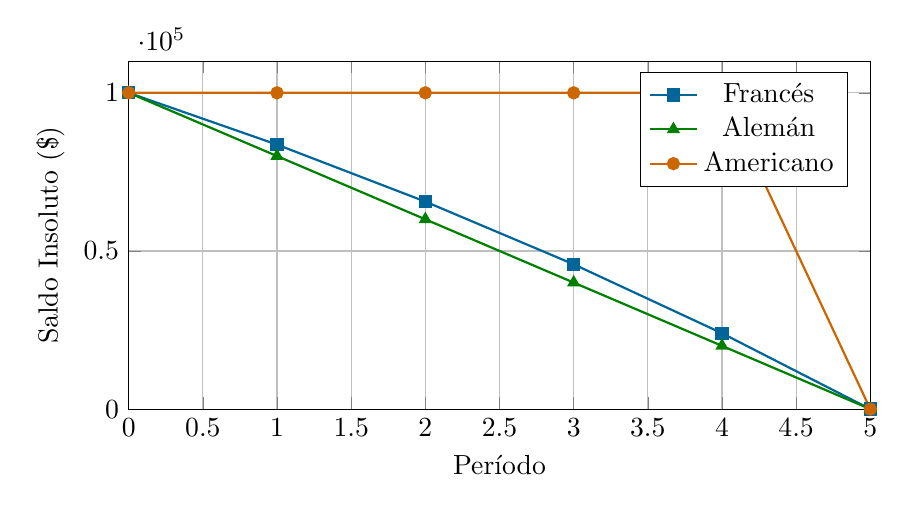
\begin{tikzpicture}
            \begin{axis}[
                xlabel={Período},
                ylabel={Saldo Insoluto (\$)},
                xmin=0, xmax=5,
                ymin=0, ymax=110000,
                grid=major,
                width=11cm,
                height=6cm,
                legend pos=north east
            ]
            % Francés
            \addplot[color=primaryblue, thick, mark=square*] coordinates {(0,100000) (1,83620) (2,65603) (3,45783) (4,23982) (5,0)};
            \addlegendentry{Francés}
            % Alemán
            \addplot[color=accentgreen, thick, mark=triangle*] coordinates {(0,100000) (1,80000) (2,60000) (3,40000) (4,20000) (5,0)};
            \addlegendentry{Alemán}
            % Americano
            \addplot[color=accentorange, thick, mark=*] coordinates {(0,100000) (1,100000) (2,100000) (3,100000) (4,100000) (5,0)};
            \addlegendentry{Americano}
            \end{axis}
        \end{tikzpicture}
    \end{center}
\end{frame}

\begin{frame}{Resumen Comparativo}
    \begin{center}
    \scriptsize
    \begin{tabular}{@{}lccc@{}}
        \toprule
        \textbf{Característica} & \textbf{Francés} & \textbf{Alemán} & \textbf{Americano} \\
        \midrule
        Cuota & Constante & Decreciente & Solo interés + bullet \\
        Amortización capital & Creciente & Constante & Todo al final \\
        Interés por período & Decreciente & Decreciente & Constante \\
        Interés total & Medio & Menor & Mayor \\
        Pago inicial & Medio & Mayor & Menor \\
        Pago final & Medio & Menor & Muy alto \\
        Saldo insoluto & Curvo & Lineal & Constante \\
        \midrule
        \textbf{Uso típico} & Hipotecas & Corporativo & Bonos \\
        \bottomrule
    \end{tabular}
    \end{center}

    \pause
    \vspace{0.3cm}

    \begin{alertblock}{¿Cuál es mejor?}
        Depende del contexto: flujo de caja del deudor, expectativas de refinanciamiento, y preferencias de liquidez.
    \end{alertblock}
\end{frame}

% ===========================================
% SECCIÓN 7: TRUCOS Y HP 17bII+
% ===========================================
\section{Trucos de Estimación Mental}

\begin{frame}{Estimación del Interés Total (Francés)}
    \begin{alertblock}{Regla práctica}
        Para un préstamo a cuota fija, el interés total es aproximadamente:
        \[
        \text{Interés total} \approx \frac{PV \times r \times (n+1)}{2}
        \]
    \end{alertblock}

    \pause
    \vspace{0.3cm}

    \textbf{Ejemplo:} \$100,000 al 10\% por 5 años

    \begin{align*}
        \text{Interés} &\approx \frac{100,000 \times 0.10 \times 6}{2} = \$30,000
    \end{align*}

    Exacto: \$31,899. Error: 6\% (aceptable para estimación rápida).

    \pause
    \vspace{0.3cm}

    \begin{exampleblock}{Por qué funciona}
        Es el promedio de pagar interés sobre el saldo completo y sobre cero.
    \end{exampleblock}
\end{frame}

\begin{frame}{Proporción de Capital en el Primer Pago}
    \begin{alertblock}{Estimación del capital inicial}
        El capital amortizado en el primer pago es aproximadamente:
        \[
        A_1 \approx \frac{PV}{n} \times \left(1 - \frac{r \times n}{2}\right)
        \]

        O más simple: si la cuota es $PMT$ y el interés del primer mes es $I_1 = PV \times r$:
        \[
        A_1 = PMT - I_1
        \]
    \end{alertblock}

    \pause
    \vspace{0.3cm}

    \textbf{Ejemplo:} Préstamo de \$300,000 a 1\% mensual, 360 meses

    $PMT \approx \$3,086$ (calculado)

    $I_1 = 300,000 \times 0.01 = \$3,000$

    $A_1 = 3,086 - 3,000 = \$86$ (solo 2.8\% de la cuota va a capital)
\end{frame}

\section{Calculadora HP 17bII+}

\begin{frame}{HP 17bII+: Funciones de Amortización}
    \textbf{Ruta:} \texttt{FIN} $\to$ \texttt{TVM} $\to$ (calcular PMT) $\to$ \texttt{OTHER} $\to$ \texttt{AMRT}

    \vspace{0.3cm}

    \begin{center}
    \begin{tabular}{@{}cl@{}}
        \toprule
        \textbf{Tecla (soft key)} & \textbf{Función} \\
        \midrule
        \texttt{\#P} & Número de pagos a amortizar \\
        \texttt{INT} & Muestra interés acumulado \\
        \texttt{PRIN} & Muestra capital amortizado \\
        \texttt{BAL} & Muestra saldo insoluto \\
        \texttt{NEXT} & Avanza al siguiente grupo de pagos \\
        \bottomrule
    \end{tabular}
    \end{center}

    \pause
    \vspace{0.3cm}

    \textbf{Procedimiento:}
    \begin{enumerate}
        \item Ingresar datos del préstamo en TVM (PV, I\%YR, N, calcular PMT)
        \item Entrar a \texttt{OTHER} $\to$ \texttt{AMRT}
        \item Ingresar número de pagos con \texttt{\#P}
        \item Presionar \texttt{INT}, \texttt{PRIN}, \texttt{BAL} según se necesite
        \item Usar \texttt{NEXT} para avanzar al siguiente bloque
    \end{enumerate}
\end{frame}

\begin{frame}{HP 17bII+: Ejemplo de Amortización}
    \begin{block}{Problema}
        Préstamo de \$50,000, 12 meses, 1.5\% mensual. ¿Cuánto interés y capital se paga en los primeros 3 meses?
    \end{block}

    \pause
    \vspace{0.2cm}

    \begin{center}
    \scriptsize
    \begin{tabular}{@{}lll@{}}
        \toprule
        \textbf{Teclas} & \textbf{Display} & \textbf{Descripción} \\
        \midrule
        \texttt{FIN} $\to$ \texttt{TVM} & & Entrar al menú TVM \\
        \texttt{CLEAR DATA} & 0.00 & Limpiar \\
        \texttt{50000 PV} & 50,000 & Préstamo \\
        \texttt{12 N} & 12 & Meses \\
        \texttt{1.5 I\%YR} & 1.5 & Tasa mensual \\
        \texttt{0 FV} & 0 & Sin valor residual \\
        \texttt{PMT} & -4,607.08 & Pago mensual \\
        \texttt{OTHER} $\to$ \texttt{AMRT} & & Entrar a amortización \\
        \texttt{3 \#P} & 3 & Amortizar 3 pagos \\
        \texttt{INT} & -2,111.14 & Interés meses 1-3 \\
        \texttt{PRIN} & -11,710.09 & Capital meses 1-3 \\
        \texttt{BAL} & 38,289.91 & Saldo después de 3 pagos \\
        \bottomrule
    \end{tabular}
    \end{center}
\end{frame}

\begin{frame}{HP 17bII+: Saldo en Cualquier Momento}
    \begin{block}{Problema}
        Mismo préstamo. ¿Cuál es el saldo después del pago 8?
    \end{block}

    \pause
    \vspace{0.3cm}

    \textbf{Método 1: Continuar amortizando}

    (Después de los 3 primeros, presionar \texttt{NEXT}...)
    \begin{center}
    \begin{tabular}{@{}lll@{}}
        \texttt{5 \#P} & 5 & Amortizar pagos 4-8 \\
        \texttt{INT} & -1,486.45 & Interés meses 4-8 \\
        \texttt{BAL} & 16,755.27 & Saldo después de pago 8 \\
    \end{tabular}
    \end{center}

    \pause
    \vspace{0.3cm}

    \textbf{Método 2: Fórmula directa}

    Quedan 4 pagos:
    \begin{align*}
        \text{Saldo}_8 = 4,607.08 \times \frac{1-(1.015)^{-4}}{0.015} = 4,607.08 \times 3.854 = \$17,755.40
    \end{align*}

    (Diferencia por redondeo)
\end{frame}

% ===========================================
% SECCIÓN 8: EJERCICIOS PRÁCTICOS
% ===========================================
\section{Ejercicios Prácticos}

\begin{frame}{Ejercicio 1: Préstamo Hipotecario}
    \begin{block}{Problema}
        Hipoteca de \$2,000,000 a 15 años, 9\% anual con pagos mensuales. Calcular:
        \begin{enumerate}
            \item Pago mensual
            \item Interés y capital del primer pago
            \item Saldo después de 5 años
        \end{enumerate}
    \end{block}

    \pause
    \vspace{0.2cm}

    \textbf{Datos:} $n = 180$ meses, $r = 0.75\%$ mensual

    \pause
    \textbf{1. Pago mensual:}
    $PMT = 2,000,000 \times \frac{0.0075}{1-(1.0075)^{-180}} = \$20,284.92$

    \pause
    \textbf{2. Primer pago:}
    $I_1 = 2,000,000 \times 0.0075 = \$15,000$
    $A_1 = 20,284.92 - 15,000 = \$5,284.92$

    \pause
    \textbf{3. Saldo después de 60 pagos (quedan 120):}
    $\text{Saldo}_{60} = 20,284.92 \times \frac{1-(1.0075)^{-120}}{0.0075} = \$1,587,614$
\end{frame}

\begin{frame}{Ejercicio 2: Sistema Alemán}
    \begin{block}{Problema}
        Préstamo de \$60,000 a 4 años, 8\% anual, sistema alemán. Calcular el pago del año 3.
    \end{block}

    \pause
    \vspace{0.3cm}

    \textbf{Amortización anual:}
    \begin{align*}
        A = \frac{60,000}{4} = \$15,000
    \end{align*}

    \pause
    \textbf{Saldo al inicio del año 3:}
    \begin{align*}
        \text{Saldo}_2 = 60,000 - 2 \times 15,000 = \$30,000
    \end{align*}

    \pause
    \textbf{Interés del año 3:}
    \begin{align*}
        I_3 = 30,000 \times 0.08 = \$2,400
    \end{align*}

    \pause
    \textbf{Pago del año 3:}
    \begin{align*}
        \text{Pago}_3 = A + I_3 = 15,000 + 2,400 = \$17,400
    \end{align*}
\end{frame}

\begin{frame}{Ejercicio 3: Comparación de Intereses}
    \begin{block}{Problema}
        Préstamo de \$80,000 a 3 años, 12\% anual. Calcular el interés total bajo cada sistema.
    \end{block}

    \pause
    \vspace{0.2cm}

    \textbf{Sistema Francés:}

    $PMT = 80,000 \times \frac{0.12}{1-(1.12)^{-3}} = \$33,309.76$

    Interés total $= 3 \times 33,309.76 - 80,000 = \$19,929.28$

    \pause
    \textbf{Sistema Alemán:}

    $I_1 = 80,000 \times 0.12 = 9,600$; $I_2 = 53,333 \times 0.12 = 6,400$; $I_3 = 26,667 \times 0.12 = 3,200$

    Interés total $= 9,600 + 6,400 + 3,200 = \$19,200$

    \pause
    \textbf{Sistema Americano:}

    Interés total $= 3 \times 80,000 \times 0.12 = \$28,800$
\end{frame}

\begin{frame}{Ejercicio 4: Pago Anticipado}
    \begin{block}{Problema}
        Tienes un préstamo de \$100,000 a 10 años, 10\% anual, cuota fija. Después del pago 5, haces un abono extra de \$20,000. ¿Cómo cambia la situación si reduces el plazo manteniendo la cuota?
    \end{block}

    \pause
    \vspace{0.2cm}

    \textbf{Cuota original:} $PMT = 100,000 \times \frac{0.10}{1-1.10^{-10}} = \$16,274.54$

    \pause
    \textbf{Saldo después del pago 5:}
    $\text{Saldo}_5 = 16,274.54 \times \frac{1-1.10^{-5}}{0.10} = \$61,698$

    \pause
    \textbf{Nuevo saldo después del abono:}
    $\text{Saldo nuevo} = 61,698 - 20,000 = \$41,698$

    \pause
    \textbf{Nuevo plazo (manteniendo cuota):}
    $n = \frac{\ln(16,274.54) - \ln(16,274.54 - 41,698 \times 0.10)}{\ln(1.10)} = 3.05$ años

    El préstamo se liquida en $\approx$ 3 años más (8 años total vs. 10 original).
\end{frame}

% ===========================================
% SECCIÓN 9: PYTHON
% ===========================================
\section{Python con numpy-financial}

\begin{frame}[fragile]{Python: Tabla de Amortización Francesa}
    \begin{lstlisting}[style=pythonstyle]
import numpy_financial as npf

def tabla_frances(pv, r, n):
    pmt = -npf.pmt(r, n, pv)
    saldo = pv

    print(f"Prestamo: ${pv:,.2f} | Tasa: {r*100:.2f}% | Periodos: {n}")
    print(f"Cuota: ${pmt:,.2f}")
    print("-" * 60)
    print("Per |   Pago    |  Interes  |  Capital  |   Saldo")
    print("-" * 60)

    total_int = 0
    for t in range(1, n+1):
        interes = saldo * r
        capital = pmt - interes
        saldo -= capital
        total_int += interes
        print(f"{t:3} | ${pmt:9,.2f} | ${interes:9,.2f} | ${capital:9,.2f} | ${max(saldo,0):10,.2f}")

    print("-" * 60)
    print(f"Total intereses: ${total_int:,.2f}")

tabla_frances(100000, 0.10, 5)
    \end{lstlisting}
\end{frame}

\begin{frame}[fragile]{Python: Componentes con numpy-financial}
    \begin{lstlisting}[style=pythonstyle]
import numpy_financial as npf

pv = 100000
r = 0.10
n = 5

# Calcular pago
pmt = -npf.pmt(r, n, pv)
print(f"Pago anual: ${pmt:,.2f}")

# Interes de cada periodo
for t in range(1, n+1):
    ipmt = -npf.ipmt(r, t, n, pv)  # Interes periodo t
    ppmt = -npf.ppmt(r, t, n, pv)  # Capital periodo t
    print(f"Año {t}: Interes=${ipmt:,.2f}, Capital=${ppmt:,.2f}")

# Saldo insoluto despues del periodo 3
saldo_3 = npf.pv(r, n-3, -pmt, 0)
print(f"\nSaldo despues de pago 3: ${-saldo_3:,.2f}")
    \end{lstlisting}
\end{frame}

\begin{frame}[fragile]{Python: Comparación de Sistemas}
    \begin{lstlisting}[style=pythonstyle]
import matplotlib.pyplot as plt
import numpy as np

pv, r, n = 100000, 0.10, 5

# Sistema Frances
pmt_f = pv * r / (1 - (1+r)**-n)
saldo_f = [pv]
for t in range(n):
    saldo_f.append(saldo_f[-1]*(1+r) - pmt_f)

# Sistema Aleman
A = pv / n
saldo_a = [pv - t*A for t in range(n+1)]

# Sistema Americano
saldo_am = [pv]*n + [0]

plt.figure(figsize=(10, 5))
plt.plot(range(n+1), saldo_f, 'b-o', label='Frances')
plt.plot(range(n+1), saldo_a, 'g-s', label='Aleman')
plt.plot(range(n+1), saldo_am, 'r-^', label='Americano')
plt.xlabel('Periodo'); plt.ylabel('Saldo')
plt.title('Comparacion de Saldo Insoluto')
plt.legend(); plt.grid(True)
    \end{lstlisting}
\end{frame}

% ===========================================
% SECCIÓN 10: RESUMEN Y TAREA
% ===========================================
\section{Resumen y Tarea}

\begin{frame}{Resumen de Fórmulas}
    \textbf{Sistema Francés:}
    \begin{align*}
        PMT &= PV \cdot \frac{r}{1-(1+r)^{-n}} \\
        \text{Saldo}_k &= PMT \cdot \frac{1-(1+r)^{-(n-k)}}{r}
    \end{align*}

    \textbf{Sistema Alemán:}
    \begin{align*}
        A &= \frac{PV}{n} \quad \text{(constante)} \\
        \text{Saldo}_t &= PV \cdot \left(1 - \frac{t}{n}\right)
    \end{align*}

    \textbf{Sistema Americano:}
    \begin{align*}
        \text{Pago periódico} &= PV \times r \\
        \text{Pago final} &= PV \times (1 + r)
    \end{align*}
\end{frame}

\begin{frame}{Conceptos Clave}
    \begin{enumerate}
        \item \textbf{Amortización} = proceso de pago de deuda
        \item Cada pago tiene componente de \textbf{interés} y \textbf{capital}
        \item \textbf{Francés}: cuota fija, más usado
        \item \textbf{Alemán}: amortización constante, menos interés total
        \item \textbf{Americano}: solo interés + bullet, más interés total
        \item El \textbf{saldo insoluto} = VP de pagos restantes
        \item HP 17bII+: \texttt{OTHER} $\to$ \texttt{AMRT} para desglose
    \end{enumerate}
\end{frame}

\begin{frame}{Tarea para la Próxima Sesión}
    \begin{enumerate}
        \item \textbf{Tabla de amortización:} Construye la tabla completa para un préstamo de \$50,000 a 6 meses, 2\% mensual, sistema francés.

        \vspace{0.3cm}

        \item \textbf{Comparación:} Para el mismo préstamo, calcula el interés total bajo los tres sistemas.

        \vspace{0.3cm}

        \item \textbf{HP 17bII+:} Usa \texttt{OTHER} $\to$ \texttt{AMRT} para verificar el interés de los primeros 3 meses del ejercicio anterior.

        \vspace{0.3cm}

        \item \textbf{Python:} Crea una función que genere la tabla de amortización para cualquiera de los tres sistemas, según un parámetro de entrada.
    \end{enumerate}
\end{frame}

% ===========================================
% CIERRE
% ===========================================

\begin{frame}
    \begin{center}
        \Huge \textcolor{primaryblue}{\textbf{¿Preguntas?}}

        \vspace{1cm}
        \Large Próxima Sesión:\\
        \textbf{Valuación de Bonos}

        \vspace{0.5cm}
        \normalsize Semana 4, Clase 2
    \end{center}
\end{frame}

\end{document}
